% !TEX root = ./main.tex

\textbf{Results}

\textbf{Complementary Transitions Implies Hydrophobic Effect}

How do MSMs from solvent coordinates match up with the protein centric view? Solvent and protein transitions are found to be interconnected, such that when mapping each set of input features to the first two slowest-relaxing tICA components there exists overwhelming similarities. Potential energy wells overlap for the two largest tICA components, tIC1 and tIC2. Furthermore, the metastable states that correspond to these basins are identical for both tICA landscapes. Many have proposed various roles for water molecules, such as water enslaving protein motions \cite{bellissent2016water}. Here, in fine detail the latter proposal was scrutinized by exposing the solvent shells that contributed to the slowest motions in the de-wetting process and emphasizing theconsequence of solvent density within the binding site.

Previously, the protein centric viewpoint of binding has been revealed. In this work, we reconstructed the protein centric MSM and built an MSM using solvent features to investigate the role of water. The same model parameters were used to objectively compare our models. A side-by-side comparison of the two tICA landscapes can be found in Figure \ref{fig:tica_compare} and implied timescales in Figure \ref{fig:implied_timescales}. The first model was built from protein pair-distances and the other using a solvent shell features metric. Remarkably, by randomly extracting clusters from the tICA subspace (Figure \ref{fig:tica_compare}) at each quadrant, we revealed that the four main metastable states coincide with findings from Zhou et al. and are as follows: top left represents the unbound-unfolded, bound-unfolded in the top right, bound-folded in the bottom right, bottom left is the bound-unfolded.

The similarities do not end here. The correlation with Tryptophan, W23 of p53, and tIC2
still exists in the solvent MSM. It has been found that trajectories that start at (+tIC1, +tIC2), and finish at the native state (+tIC1, -tIC2) predominantly display W23 facing out of the page when looking at MDM2-p53 from the orientation shown in all the figures from this work. Likewise, trajectories starting at (-tIC1, -tIC2) show W23 oriented into the page.  An observed trend impossible to detect from the protein centric model shows that post binding of MDM2-p53, bundles of water is commonly found to associate—requiring an increase of water fluctuation to induce burrowing of W23.


The second component (tIC2) is related to the first component, which directly corresponds to de-wetting. When moving from -tIC1 to +tIC1, we find a
direct correlation in the number of water molecules inside the pocket, corresponding to the proximity of p53 to MDM2's binding site, where the location of the native state resides in (+tIC1,-tIC2) of the tICA landscape. Naturally, as bulky residues enter the hydrophobic pocket, water tends to relocate to find more polar interactions. For example, as greasy tryptophan (W23) enters the pocket with or without the correct orientation, there is a positive shift along tIC1, and stability of the bound alpha helix is maximized when W23 is in the correct orientation (into page). Phenylanine (F19) also induces a positive shift along tIC1 as it buries regardless of W23's orientation (+tIC1, ±tIC2).

\textbf{Slowest-dyanmical Solvent Features}

Solvent shell featurization achieves instantaneous solvent density with
respect to solvent features over all trajectories \cite{harrigan2015conserve}. Solvent features are binned water molecules from considering only solute-solvent distances. The 63 solute atoms ($C_{\alpha}$'s and $C_{\beta}$'s) each contain 4 equidistant shells around them giving 252 solvent features.
%Information regarding specific shells must be taken from the eigenvector, which requires decomposition to investigate each of the shells with respect to specific solute atoms.
The feature vector yields information over all trajectories and was transformed by tICA to produce a linear combination of water features. After construction of the 10-component tICA model, which serves as the new basis set for the data, we subsequently built a
solvent MSM following equivalent parameters as Zhou et al.

Information regarding individual solvent features that correlate to the slowest-dynamical motions of de-wetting were extracted from the 1\textsuperscript{st} eigenvector. From this, mechanism is determined.  The important solvent features are represented as a color map shown in the bottom panel of Figure \ref{fig:1st_eigenvector}, moving from negative (pink) to positive (yellow).  The color represents the degree of contribution to the slowest dynamical solvent motions within a specific shell. The coefficients used to represent this magnitude comes from the normalized 1\textsuperscript{st} eigenvector to elude from noise (top panal of Figure \ref{fig:1st_eigenvector}).


The residues with the greatest contributions to the slow motions of de-wetting are shown in Figure \ref{fig:atom_indices} and have been colored accordingly for a convenient reference.  The slow-dynamical solvent features included the first shell (0-3 Å) of Histidine, H73 ($\alpha$) and Glutamine, Q72 ($\alpha$, $\beta$) of MDM2 along with the second shell (3-6 Å) of K24($\alpha$, $\beta$) and T18($\alpha$, $\beta$) of p53.




\begin{figure}[h!]
\centering
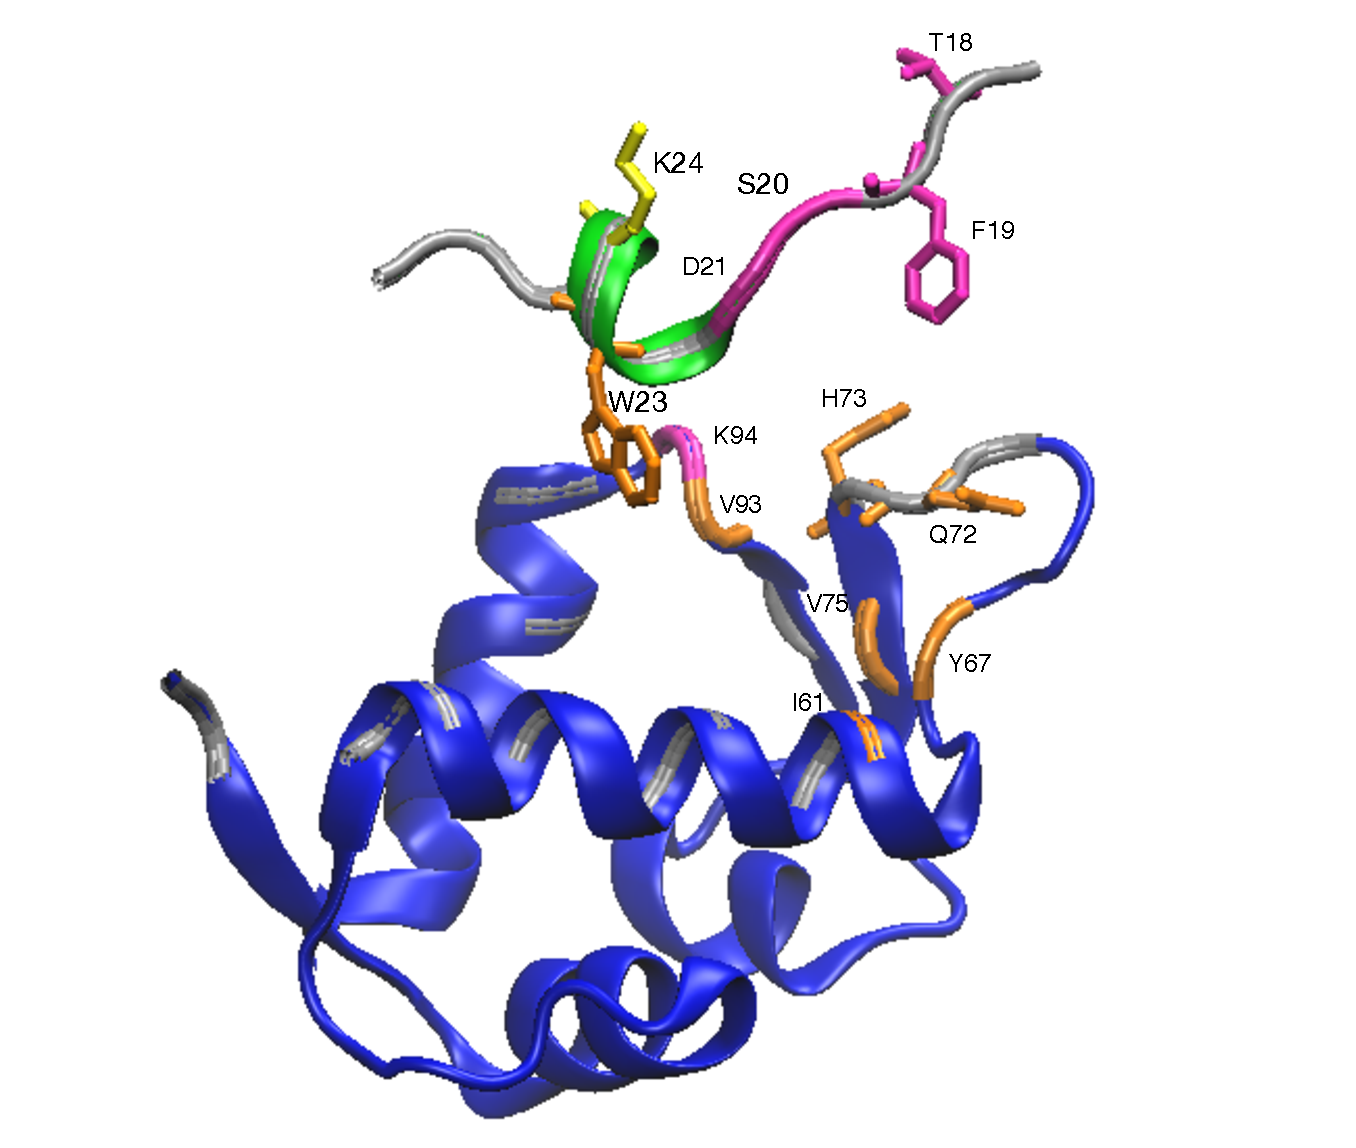
\includegraphics[scale=0.5]{Figures/Structure/Atom_indices_with_1st_eigenvector_sel.pdf}
\caption{MDM2 (blue) and p53 (green) shown with residues (silver, orange, pink, and yellow) containing $C_{\alpha}$ and $C_{\beta}$ solute atoms selected for water shell featurization. Significant residues are identified from the normalized squared components of the 1\textsuperscript{st} eigenvector (see Figure \ref{fig:1st_eigenvector}) and colored accordingly.}
\label{fig:atom_indices}
\end{figure}


\begin{figure}[h!]
\centering
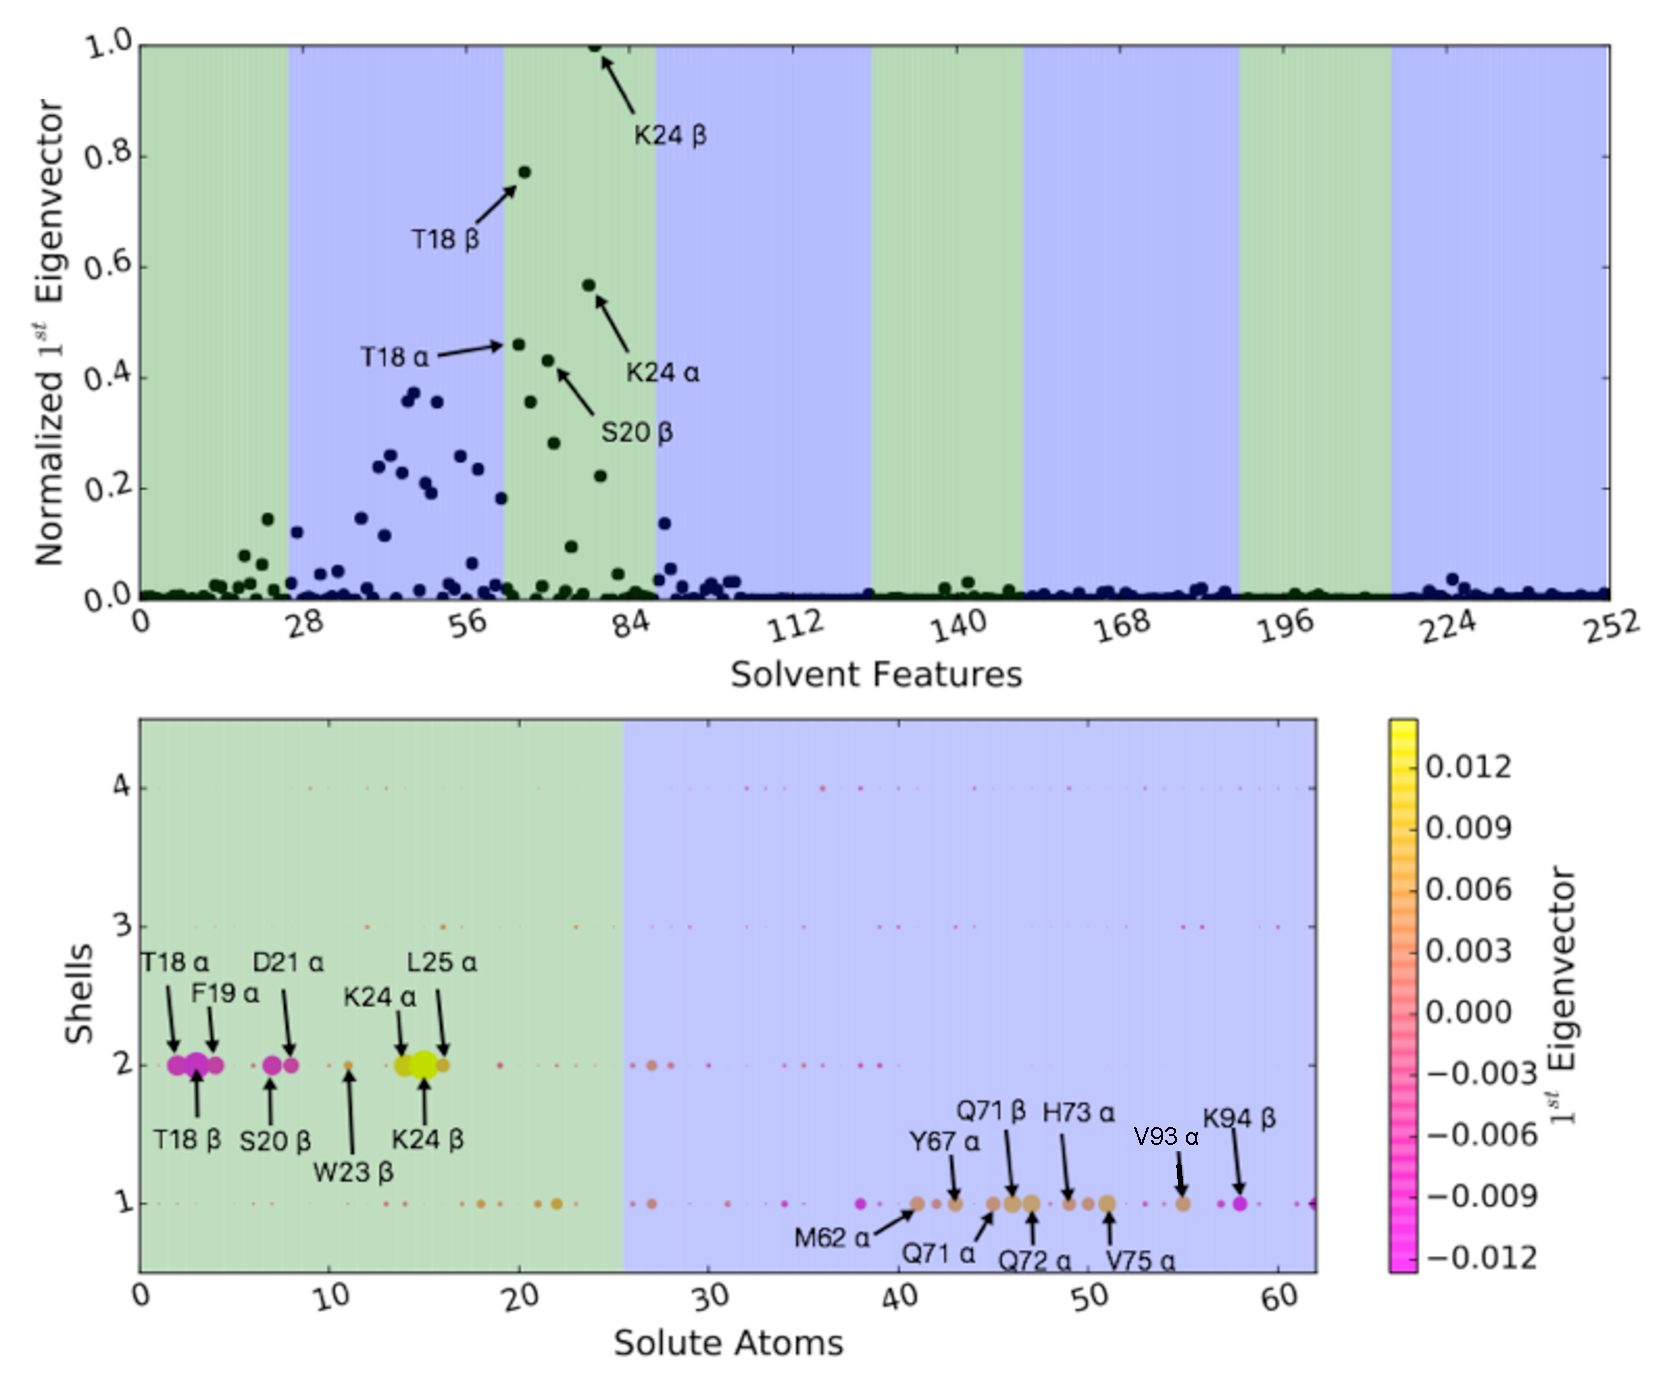
\includegraphics[scale=0.5]{Figures/SolvShellFeatures/Solvent_Shell_Feature_Eigen_1.pdf}
\caption{\textbf{Solvent shells around key residues contribute to the slowest de-wetting motions.} (Top) The degree of contribution for each solvent shell. Significant slow-dynamical solvent features are labeled for important solute atoms ($C_{\alpha}$ and $C_{\beta}$). The first 26 features are of the first shell of p53 (green), then the next 38 are of the first shell of MDM2 (blue). Next, second shell of p53, and so on. (Bottom) Transformed eigenvector to show individual shell contribution. The color map represents the slow solvent dynamics of the system as it relaxes towards equilibrium (pink to yellow).}
\label{fig:1st_eigenvector}
\end{figure}


Using the solvent shell metric associated with the greatest magnitude of importance (3-6 Å of p53) the waters within this region were highlighted and traced along specific trajectories. In addition to this quantitative approach, instantaneous (1 ns) solvent density was qualitatively uncovered with the help of Chimera's MolMap. At each instant along a trajectory an occupancy surface was gen rated to clearly represent the absence of water-oxygens. As one would expect, an inverse relationship was found for the proximity of p53 to MDM2 and the number of water-oxygens in the vicinity of the pocket.

The tICA landscape in Figure \ref{fig:tica} was generated with solvent shell input features. Overlaid on this 2-D landscape is a trajectory with a duration of 531 ns that spans the majority of tIC1. This particular trajectory undergoes five transitions (a)-(e) where each transition is represented with a snapshot that has been hand selected from the 600 clusters. See the supplemental information section for this trajectory, as well as five additional trajectories (movies) which span all of the quadrants of the tICA landscape.

Four main transition states can be seen in this trajectory, starting from the bound-unfolded ending up into the bound-folded state. This trajectory is consistent with the "fly-casting" mechanism, in that threonine, T18 (cyan) and phenylanine, F19 (light green) of p53 enter the pocket first displacing some transient water molecules, but large surface cavities still exist (a-b). The next transition state (c) occurs at 201 ns (00:07) where W23 (yellow) enters the pocket. Here, expropriation of space by bulky Tryptophan of p53 displaces a large water cluster from the pocket forcing reorganization of water molecules (c). It is the fluctuation of water that assists W23 for a deep insertion into the pocket at 308 ns (00:10). In turn, p53 is pulled down which contorts the alpha helix with a torque screw motion throwing threonine T18 upwards, (d) simultaneously enabling F19 to dig down into the cleft at 314 ns (00:11). In the last transition (e), F19 and W23 hold a strong foundation and maintain alpha helix stability by hydrogen bonds. Solvent eventually makes the environment around K24 chaotic enough to complete the loop for a complete fully structured alpha helix.

\begin{figure}[h!]
\centering
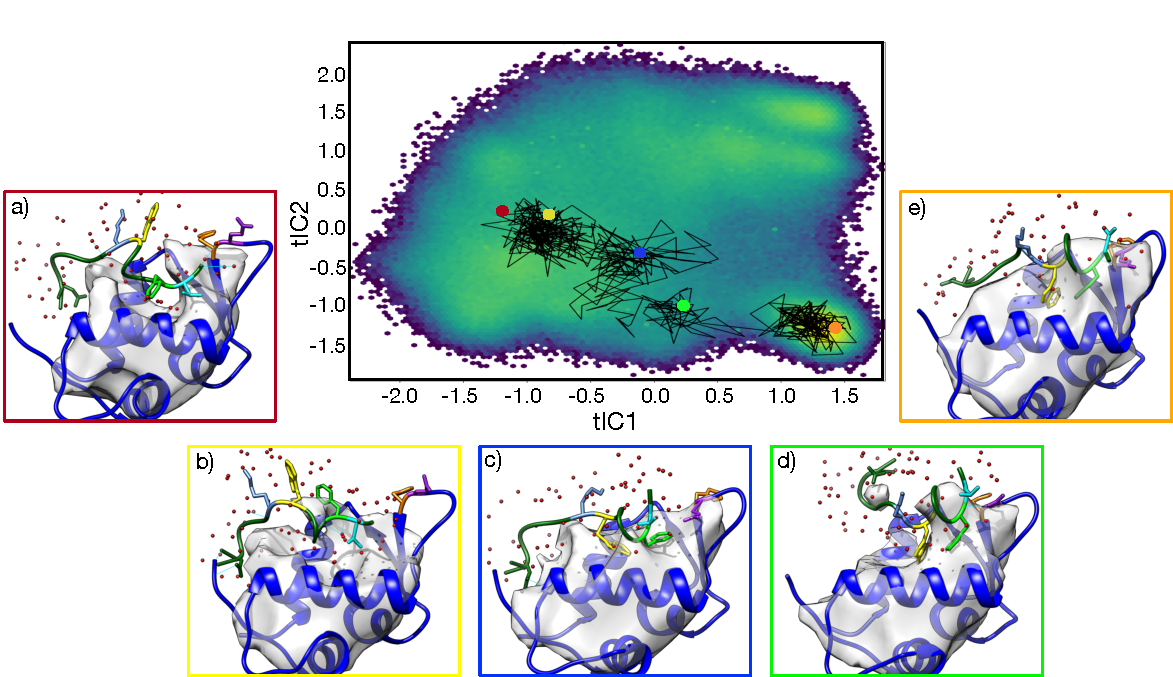
\includegraphics[scale=0.75]{Figures/Partitioned/Partitioned_final.pdf}
\caption{\textbf{De-wetting in a protein binding trajectory.} Solvent
features projected onto a 2D tICA subspace corresponding to the first
and second components, tIC\textsubscript{1} and tIC\textsubscript{2}.~
Each color-coded snapshot represents a transition state containing its
own unique molmap (Gaussian smoothing at the 0.015 level) characterizing
instantaneous solvent density. MDM2 (blue): Q71 (purple), H72 (orange)
and p53 (green): L24 (light blue), T18 (red), F19 (pink) and W23 (cyan).}
\label{fig:tica}
\end{figure}


Water traces are displayed below for T18 and W23 of p53, which have been deemed important residues, more specifically, the 2\textsuperscript{nd} shells of each are regarded significant.  Water traces fro W23 and T18 are shown for the trajectory overlaid in Figure \ref{fig:tica}.  These water counts demonstrate that the transition from (b) to (c) are indeed coupled.


\begin{figure}[h!]
\centering
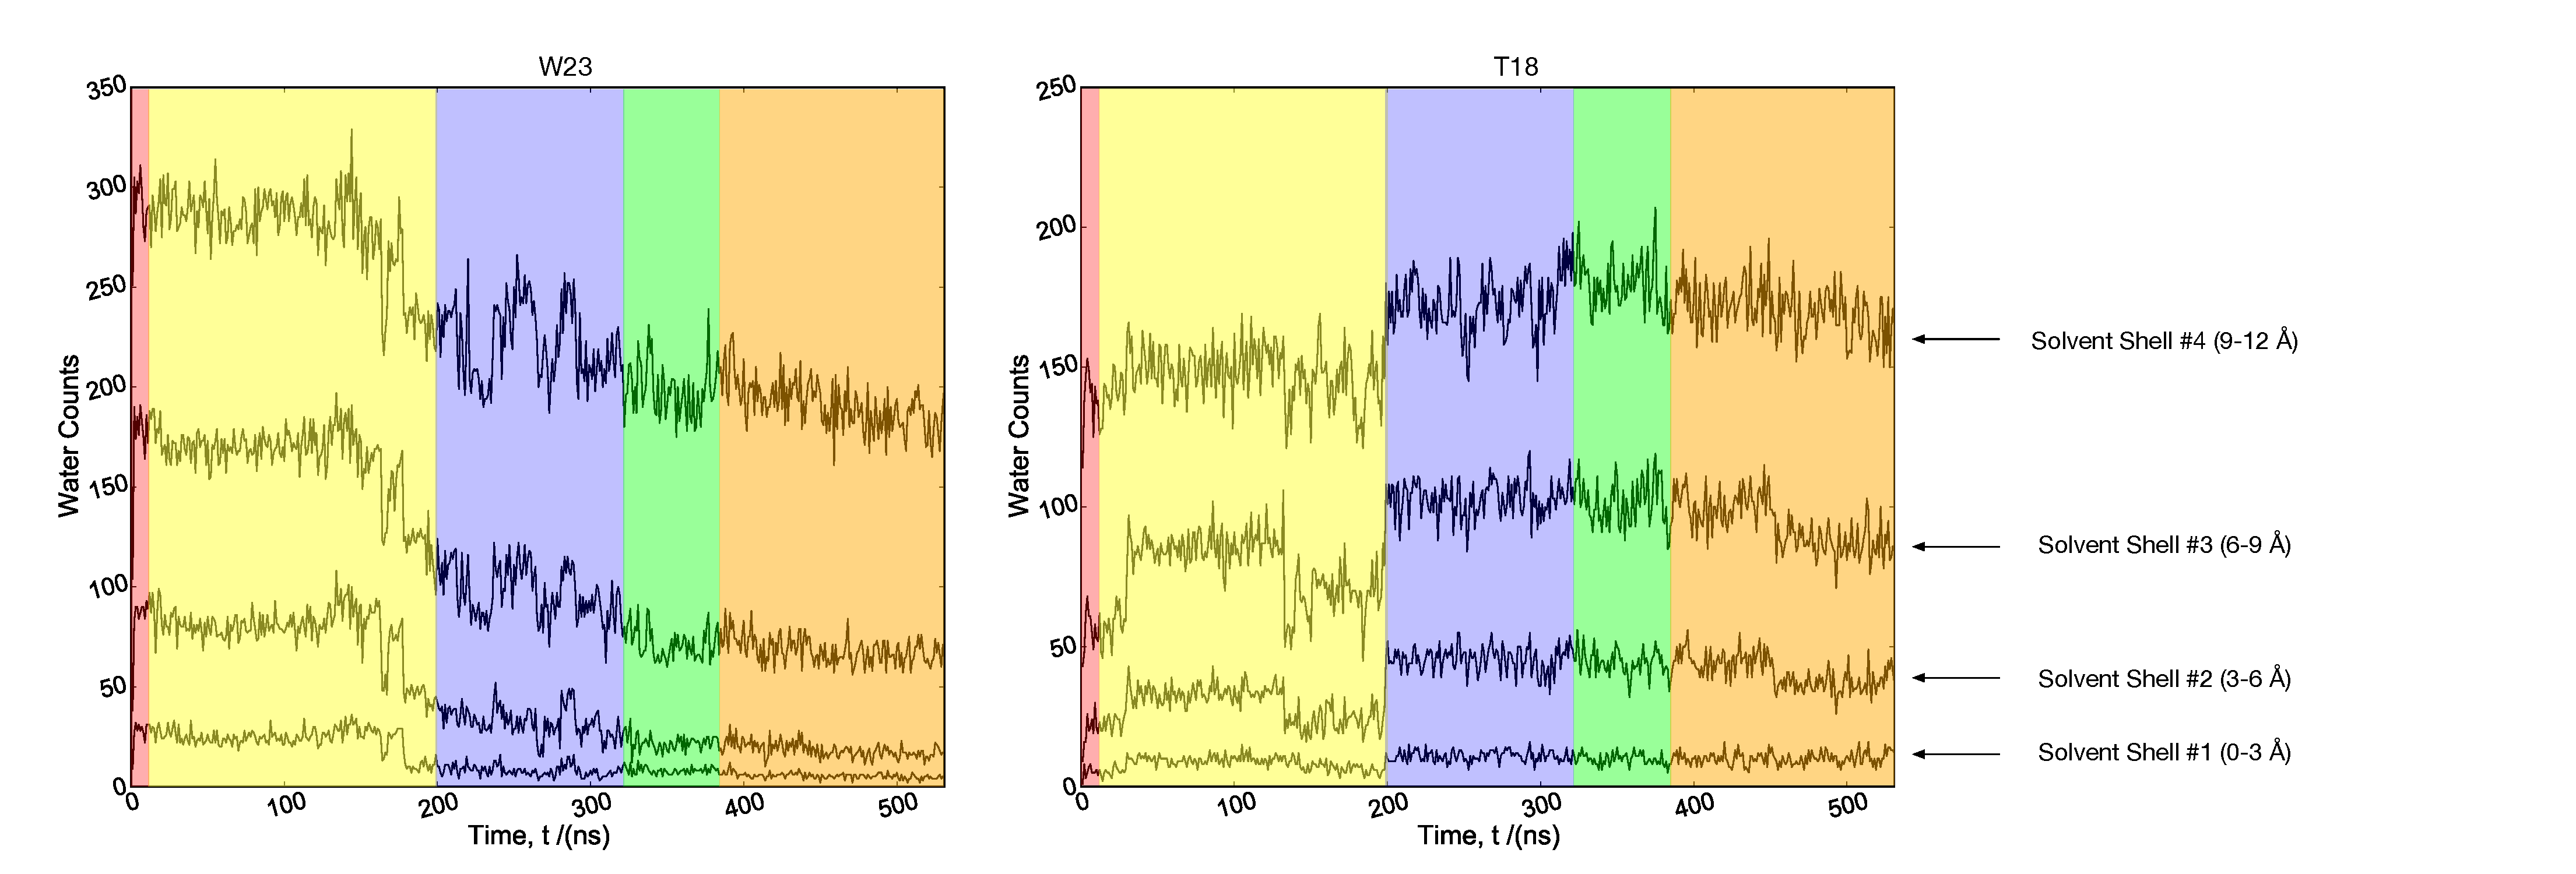
\includegraphics[scale=0.25]{Figures/Water_counts/Water_counts.pdf}
\caption{Water counts for W23 and T18 of p53 TAD,
corresponding to the trajectories shown in Figure 4. Changes in. these
observables discernibly follow the movements associated with transitions
(b)-(d).}
\label{fig:water_counts}
\end{figure}

%T18 was identified to contain significant solvent dynamics around 3-6Å.

%Instantaneous solvent density from specific movies (SI) suggests the hydrophobic effect plays a keyrole in water dynamics.

Interestingly, a recent study \cite{yadahalli2019kinetic} also notes the importance of theronine in the binding of p53 to MDM2 and suggests a ten-to twenty-fold decrease in binding affinity when Thr18 is phosporylated in comparison to the wild-type p53.  It is known that the hydrogen bond acceptor from the oxygen atom in water molecules is in fact a primary mechanism of protein stability. As an example of this, threonine T18 of p53 creates hydrogen bonds with water especially when T18 is in close proximity to Q72 of MDM2, where the jostling of water clusters back-and-forth between these two residues increases the formation of hydrogen bonds.  Water could act as an intermediate state stabilizer if found where hydrogen bonds are formed with the hydroxyl group of polar residues like T18 and Lysine, K24 to facilitate the structural transformation of the p53 $\alpha$-helix. Water bundles are found during important motions of helix formation and can be found looking for surface cavities. Scattering of water leads to reorganization to increase polar interactions and position themselves to a more favorable location.











%It is well known that water can become trapped in cavities as a result of protein binding attempts. Many transitions were found that during the binding of p53-MDM2 water would become trapped inside the hydrophobic pocket. Entrapped waters don't usually vacate until bulky nonpolar residues such as W23 and F19 of p53 form a greasy surrounding for the water molecules slip out.



